\documentclass[a4paper,14pt]{extarticle} 
\usepackage[a4paper,top=1.5cm, bottom=1.5cm, left=2cm, right=1cm]{geometry}
%\usepackage[T2A]{fontenc}
%\usepackage[english, russian]{babel}
\usepackage{graphicx}
\DeclareGraphicsExtensions{.pdf,.png,.jpg}
\usepackage{fontspec}
\setmainfont{Times New Roman}
\setsansfont{FreeSans}
\setmonofont{FreeMono}
\renewcommand{\baselinestretch}{1.5}
\usepackage{polyglossia}
\setdefaultlanguage{russian}
\setotherlanguages{english,russian}
\usepackage{setspace}
\usepackage[many]{tcolorbox}
\usepackage{listings}
\usepackage{multicol}
\usepackage{xcolor}
\usepackage{pdfpages}

\definecolor{codegreen}{rgb}{0,0.6,0}
\definecolor{codegray}{rgb}{0.5,0.5,0.5}
\definecolor{codepurple}{rgb}{0.58,0,0.82}
\definecolor{backcolour}{rgb}{0.95,0.95,0.92}

\lstdefinestyle{mystyle}{
    backgroundcolor=\color{backcolour},   
    keywordstyle=\color{magenta},
    numberstyle=\tiny\color{codegray},
    stringstyle=\color{codepurple},
    basicstyle=\ttfamily\footnotesize,
    breakatwhitespace=false,         
    breaklines=true,                 
    captionpos=b,                    
    keepspaces=true,                 
    numbers=left,                    
    numbersep=5pt,                  
    showspaces=false,                
    showstringspaces=false,
    showtabs=false,                  
    tabsize=2
}

\lstset{style=mystyle}

\begin{document}
    \begin{center}
        \thispagestyle{empty}
        \begin{singlespace}
        ФЕДЕРАЛЬНОЕ АГЕНТСТВО СВЯЗИ

        ФЕДЕРАЛЬНОЕ ГОСУДАРСТВЕННОЕ БЮДЖЕТНОЕ ОБРАЗОВАТЕЛЬНОЕ

        УЧРЕЖДЕНИЕ ВЫСШЕГО ОБРАЗОВАНИЯ

        «САНКТ-ПЕТЕРБУРГСКИЙ ГОСУДАРСТВЕННЫЙ УНИВЕРСИТЕТ ТЕЛЕКОММУНИКАЦИЙ ИМ. ПРОФ. М.А. БОНЧ-БРУЕВИЧА»

        (СПбГУТ)
        \end{singlespace}
        \vspace{-1ex}
        \rule{\textwidth}{0.4pt}
        \vspace{-5ex}

        Факультет \underline{Инфокоммуникационных сетей и систем}

        Кафедра \underline{Защищенных систем связи}
        \vspace{10ex}

        \textbf{Лабораторная работа №2}\\
        Авторизация сетевых соединений
        


    \end{center}
    \vspace{4ex}
    \begin{flushright}
    \parbox{10 cm}{
    \begin{flushleft}
        Выполнили студенты группы ИКТЗ-83:

        \underline{Громов А.А., Миколаени М.С., Мазеин Д.С.} \hfill \rule[-0.85ex]{0.1\textwidth}{0.6pt}

        \footnotesize \textit{ (Ф.И.О., № группы) \hfill (подпись)} \normalsize

        Проверил:

        \underline{Казанцев А.А.} \hfill \rule[-0.85ex]{0.1\textwidth}{0.6pt}

        (\footnotesize \textit{уч. степень, уч. звание, Ф.И.О.) \hfill (подпись)} \normalsize

    \end{flushleft}
    }
    \end{flushright}
    \begin{center}
        \vfill
        Санкт-Петербург

        2021

    \end{center}
    \newpage


    \textbf{Пункт 2 - Убедиться, что передается открытый трафик.}
    \begin{center}
        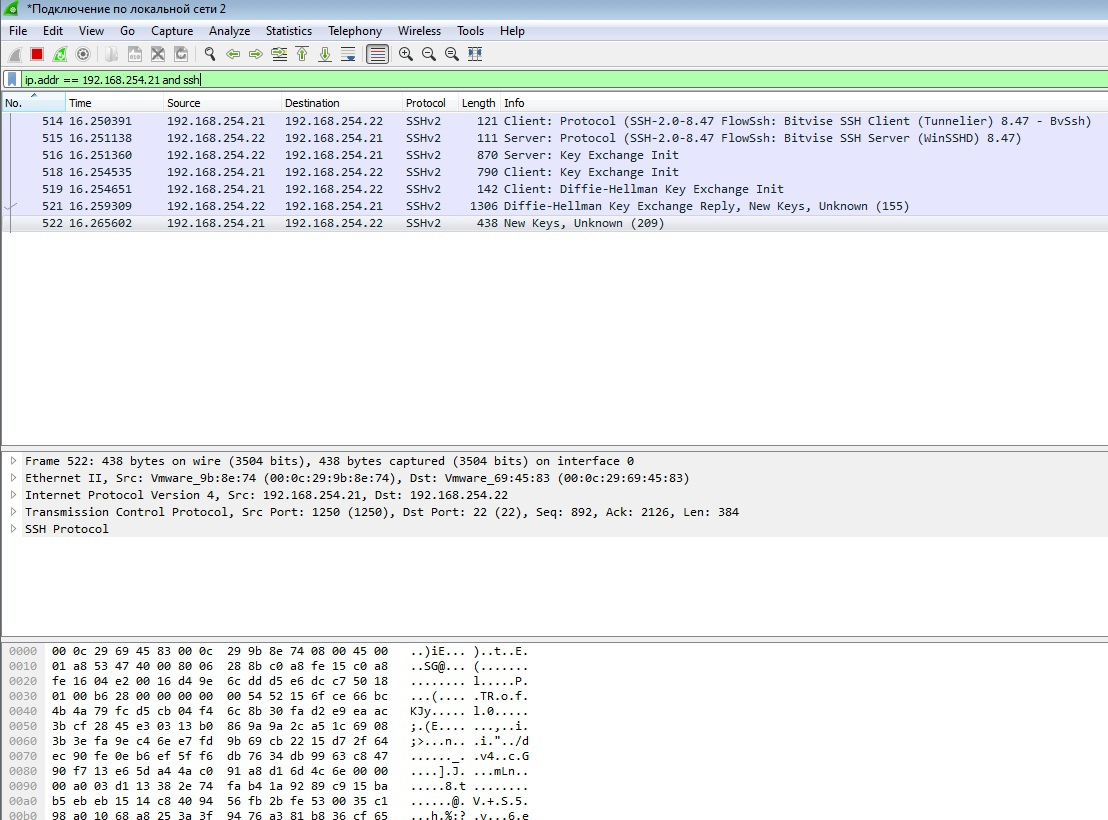
\includegraphics[scale=0.3]{pics/2.jpg}

       Открытый трафик. 
    \end{center}

    \textbf{Пункт 3 - Настройка правил доступа}
    \begin{center}
        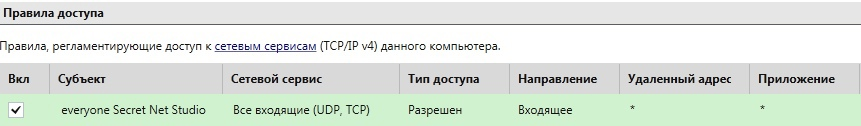
\includegraphics[scale=0.5]{pics/3.jpg}

       Парвило доступа.
    \end{center}

    \textbf{Пункт 4 - Настройка режима защиты сетевых соединений}
    \begin{center}
        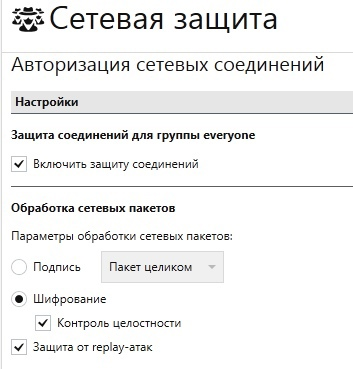
\includegraphics[scale=0.6]{pics/4.jpg}

       Экран настрокий.
    \end{center}

    \textbf{Пункт 5 - Убедиться, что передается защифрованный трафик}
    \begin{center}
        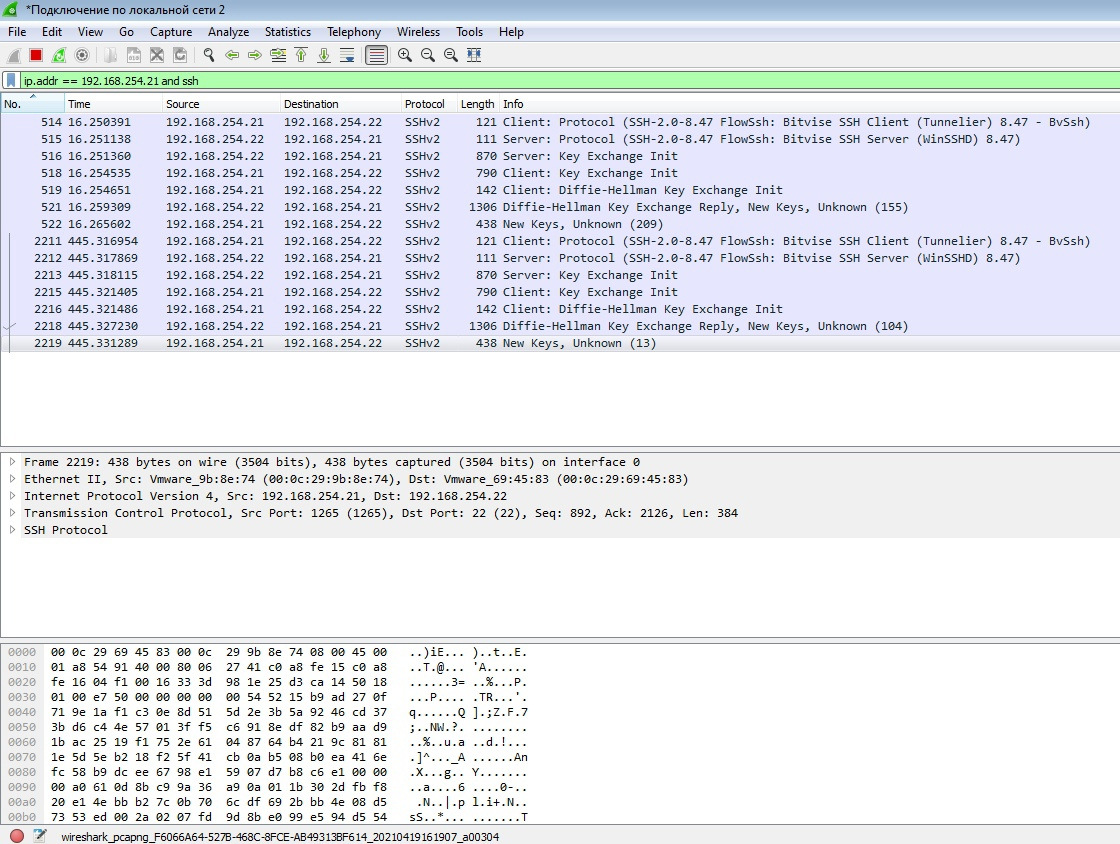
\includegraphics[scale=0.3]{pics/5.jpg}

        Не удалось защифровать трафик.
    \end{center}

    \textbf{Пункт 7 - Настройка блокировки соединений для неавторизованных на СБ пользователей}
    \begin{center}
        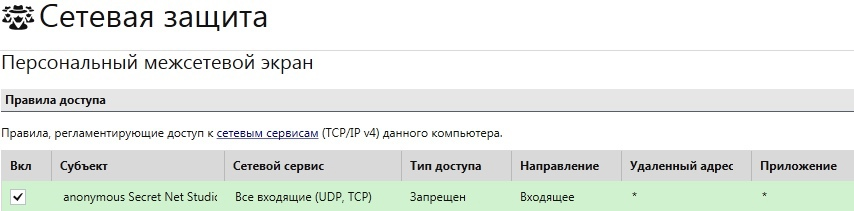
\includegraphics[scale=0.5]{pics/7.jpg}

       Парвило доступа.
    \end{center}

    \textbf{Ответы на контрольные вопросы.}

    \begin{enumerate}
        \singlespacing
        \item В отличие от традиционных, "периметровых" МЭ, реализованный в SNS \linebreak
        распределенный межсетевой экран предназначен именно для защиты \linebreak информации 
        внутри сети организации, функционирует непосредственно на ее защищаемых объектах 
        (сервер БД, рабочие места руководителей или сотрудников и т.д.) и обеспечивает 
        их защиту от сетевых угроз со стороны внешнего и внутреннего нарушителей.
        \item Правила доступа, прикладные правила, системные правила, сетевые протоколы.
        \item Системные правила
        \item Все IP-based протоколы (RDP)
        \item Прикладные правила. Регламентируют доступ пользователей к сетевым сервисам защищаемого компьютера (например, общие папки).
        \item Чем выше правило в таблице, тем больше его приоритет
        \item 4 - 6 минут
        \item Сетевой режим
        \item Механизм авторизации сетевых соединений обеспечивает защиту \linebreak взаимодействия только между авторизованными на СБ клиентами Secret Net Studio. Если на компьютере пользователя не установлен Secret Net Studio или пользователь по каким-либо причинам не прошел аутентификацию на СБ SNS (anonymous), то трафик между ним и авторизованным клиентом SNS не будет защищаться.
        \item Средствами протоколов семейства IPsec, а именно AH (Authentication Header) - гарантирует аутентичность и целостность и ESP (Encapsulation Security Payload) - шифрование и контроль целостности.
        \item Необходима лицензия на использование механизма авторизации сетевых \linebreak соединений.
        \item Если прохождение пакетов по протоколу SMB запрещается системными \linebreak правилами
        или правилами доступа, то прикладные правила не работают, так как на транспортном уровне IP-пакеты блокируются.
    \end{enumerate}
\end{document}

